\documentclass[11pt,a4paper]{article}
\usepackage[top=16mm,bottom=17mm,left=16mm,right=16mm,headheight=0pt,headsep=0mm,footskip=10mm]{geometry}
\usepackage{iftex}
\ifPDFTeX
 \usepackage[utf8]{inputenc}
 \usepackage[T5]{fontenc}
 \usepackage{mathptmx}
\else
 \usepackage{mathptmx}
 \usepackage{fontspec}
 \IfFontExistsTF{Times New Roman}{\setmainfont{Times New Roman}}{\IfFontExistsTF{TeXGyreTermes}{\setmainfont{TeXGyreTermes}}{\setmainfont{Latin Modern Roman}}}
\fi
\usepackage{amsmath,amssymb}
\usepackage{xcolor,tikz,enumitem,multicol,fancyhdr,lastpage}
\usepackage[most]{tcolorbox}
% Giu phong cach, mau sac va bo cuc cua Toan_11_04.tex.
\definecolor{questionpurple}{RGB}{137,38,143}
\definecolor{answerblue}{RGB}{35,45,140}
\definecolor{lightblue}{RGB}{238,245,255}
\setlength{\parindent}{0pt}
\setlength{\parskip}{0pt}
\renewcommand{\baselinestretch}{1.10}
\setlength{\columnsep}{8mm}
\pagestyle{fancy}
\fancyhf{}
\renewcommand{\headrulewidth}{0pt}
\fancyfoot[L]{\small Chuyên đề I -- Toán 11}
\fancyfoot[R]{\small Trang \thepage/\pageref{LastPage} -- Bài 05}
\renewcommand{\footrulewidth}{.4pt}
\setlist[itemize]{leftmargin=6mm,label=\textcolor{answerblue}{\textbullet},itemsep=2pt,topsep=3pt,parsep=0pt}
\setlist[enumerate]{leftmargin=8mm,itemsep=4pt,topsep=3pt,parsep=0pt}
\newtcolorbox{theorybox}{colback=lightblue,colframe=answerblue!60,boxrule=.5pt,
 arc=1mm,left=2.5mm,right=2.5mm,top=1.5mm,bottom=1.5mm,before skip=3pt,after skip=4pt}
\newcommand{\sectitle}[2]{\vspace{4pt}\noindent{\large\bfseries\textcolor{questionpurple}{#1.\ #2}}\par\vspace{3pt}}
\newcommand{\exampletitle}[2]{\vspace{3pt}\noindent{\bfseries\textcolor{answerblue}{Ví dụ #1.}} #2\par\vspace{2pt}}
\newcommand{\compactproblems}{\setlist[enumerate,1]{label=\textcolor{questionpurple}{\bfseries\arabic*.},leftmargin=7mm,labelsep=1.5mm,itemsep=3pt,topsep=2pt}}
\newcommand{\sinegraph}{%
 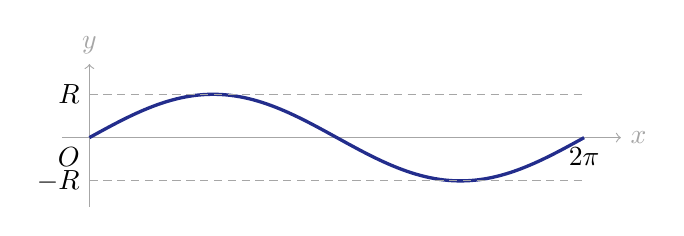
\begin{tikzpicture}[x=1.0cm,y=.55cm,baseline=(current bounding box.center)]
   \draw[->,gray!70] (-.35,0)--(6.75,0) node[right] {$x$};
   \draw[->,gray!70] (0,-1.6)--(0,1.7) node[above] {$y$};
   \draw[answerblue,very thick,domain=0:6.283,samples=110] plot (\x,{sin(\x r)});
   \draw[densely dashed,gray!70] (0,1)--(6.3,1) (0,-1)--(6.3,-1);
   \node[left] at (0,1) {$R$}; \node[left] at (0,-1) {$-R$};
   \node[below left] at (0,0) {$O$};
   \node[below] at (6.283,0) {$2\pi$};
 \end{tikzpicture}}

\begin{document}
\noindent
\begin{minipage}[t]{.35\linewidth}
 \centering{\bfseries CHUYÊN ĐỀ I -- TOÁN -- 11\par}
 \vspace{2pt}\rule{.73\linewidth}{.4pt}\par\vspace{3pt}
 CHƯƠNG I\par\vspace{3pt}{\itshape TÀI LIỆU HỌC TẬP -- BÀI 05\par}
\end{minipage}\hfill
\begin{minipage}[t]{.62\linewidth}
 \centering{\bfseries HÀM SỐ LƯỢNG GIÁC\par VÀ PHƯƠNG TRÌNH LƯỢNG GIÁC\par}
 \vspace{4pt}{\small\bfseries BÀI 05. HÀM SỐ VÀ PHƯƠNG TRÌNH\par DẠNG $a\sin x+b\cos x$\par}
\end{minipage}

\vspace{5mm}
\noindent\textbf{Họ và tên:}\dotfill\hfill\textbf{Lớp:}\enspace\dotfill
\vspace{3mm}
\begin{theorybox}
\textbf{Kiến thức trọng tâm:} Khảo sát hàm số $y=a\sin x+b\cos x$;
biến đổi thành một hàm sin hoặc cos, tìm giá trị lớn nhất, nhỏ nhất,
khoảng đồng biến, nghịch biến và giải phương trình $a\sin x+b\cos x=c$.
Giả sử $a^2+b^2\ne0$ và $k\in\mathbb Z$ trong các công thức nghiệm.
\end{theorybox}

\sectitle{1}{Khảo sát hàm số $y=a\sin x+b\cos x$}
\textbf{Công thức cộng lượng giác:}
\[
\sin(x\pm\alpha)=\sin x\cos\alpha\pm\cos x\sin\alpha,\qquad
\cos(x\pm\alpha)=\cos x\cos\alpha\mp\sin x\sin\alpha.
\]
Đặt $R=\sqrt{a^2+b^2}>0$. Khi đó
\[
 y=a\sin x+b\cos x
 =R\left(\frac{a}{R}\sin x+\frac{b}{R}\cos x\right).
\]
Vì $\left(\frac aR\right)^2+\left(\frac bR\right)^2=1$, tồn tại
$\alpha$ sao cho
\[
 \cos\alpha=\frac aR,\qquad \sin\alpha=\frac bR.
\]
\begin{theorybox}
\textbf{Đưa về một hàm lượng giác:}
\[
\boxed{y=R(\cos\alpha\sin x+\sin\alpha\cos x)
       =R\sin(x+\alpha),\quad R=\sqrt{a^2+b^2}.}
\]
\begin{itemize}
 \item \textbf{Tập xác định:} $D=\mathbb R$; hàm số tuần hoàn với chu kì $T=2\pi$.
 \item \textbf{Tập giá trị:} $[-R;R]$, hay $-R\le y\le R$.
 \item \textbf{GTLN:} $\max y=R$ khi
 $x=-\alpha+\dfrac\pi2+2k\pi$.
 \item \textbf{GTNN:} $\min y=-R$ khi
 $x=-\alpha-\dfrac\pi2+2k\pi$.
 \item \textbf{Đồng biến} trên mỗi khoảng
 $\left(-\alpha-\dfrac\pi2+2k\pi;\ -\alpha+\dfrac\pi2+2k\pi\right)$.
 \item \textbf{Nghịch biến} trên mỗi khoảng
 $\left(-\alpha+\dfrac\pi2+2k\pi;\ -\alpha+\dfrac{3\pi}{2}+2k\pi\right)$.
\end{itemize}
\end{theorybox}
\begin{center}
{\small Đồ thị minh họa của $y=R\sin x$ (dạng chuẩn sau khi tịnh tiến ngang):}\par\vspace{2pt}
\sinegraph
\end{center}

\exampletitle{01 [TDM32]}{Tìm GTLN, GTNN và các khoảng đồng biến, nghịch biến của các hàm số sau:}
\begingroup\compactproblems
\begin{enumerate}
 \item $y=\sqrt3\sin x+\cos x$.
 \item $y=\sin x-\cos x+3$.
 \item $y=-\sin2x+\sqrt3\cos2x$.
\end{enumerate}
\endgroup

\exampletitle{02 [TDM32]}{Tìm GTLN và GTNN của các hàm số sau:}
\begingroup\compactproblems
\begin{enumerate}
 \item $y=\sqrt3\sin x+4\cos x+11$.
 \item $y=4\cos^2x-2\sin x\cos x$.
 \item $y=\sqrt2\cos\!\left(x+\dfrac\pi4\right)
       +2\sin\!\left(x+\dfrac\pi6\right)$.
\end{enumerate}
\endgroup

\sectitle{2}{Phương trình lượng giác $a\sin x+b\cos x=c$}
\textbf{Bước 1.} Đặt $R=\sqrt{a^2+b^2}>0$ rồi biến đổi vế trái:
\[
 a\sin x+b\cos x
 =R\left(\frac aR\sin x+\frac bR\cos x\right).
\]
\textbf{Bước 2.} Chọn một trong hai cách đặt góc phụ:
\[
\left\{\begin{aligned}
 \cos\alpha&=\frac aR,\\
 \sin\alpha&=\frac bR
\end{aligned}\right.
\qquad\text{hoặc}\qquad
\left\{\begin{aligned}
 \sin\beta&=\frac aR,\\
 \cos\beta&=\frac bR.
\end{aligned}\right.
\]
\textbf{Bước 3.} Đưa phương trình về dạng cơ bản:
\begin{theorybox}
\[
\boxed{a\sin x+b\cos x=c
 \iff R\sin(x+\alpha)=c
 \iff \sin(x+\alpha)=\frac cR.}
\]
Hoặc tương đương
\[
\boxed{R\cos(x-\beta)=c
 \iff \cos(x-\beta)=\frac cR.}
\]
\textbf{Điều kiện phương trình có nghiệm:}
\[
\boxed{\left|\frac cR\right|\le1
 \iff |c|\le\sqrt{a^2+b^2}
 \iff a^2+b^2\ge c^2.}
\]
\end{theorybox}
\textbf{Bước 4.} Nếu thỏa điều kiện có nghiệm, giải phương trình sin
hoặc cos vừa thu được theo công thức nghiệm lượng giác cơ bản.

\exampletitle{01 [TDM32]}{Tìm điều kiện của tham số $m$ để phương trình sau có nghiệm:}
\begingroup\compactproblems
\begin{enumerate}
 \item $m\sin x+3\cos x=2m-3$.
 \item $2\cos^2x+m\sin2x=3m-4$.
\end{enumerate}
\endgroup

\exampletitle{02 [TDM32]}{Giải các phương trình lượng giác sau:}
\begingroup\compactproblems
\begin{enumerate}
 \item $\cos x-\sqrt3\sin x=2$.
 \item $\sin x+\cos x=\sqrt3$.
 \item $3\cos x+4\sin x=3$.
 \item $-3\cos2x+4\sin2x=-4$.
 \item $4\cos^2x+2\sin x\cos x=-1$.
\end{enumerate}
\endgroup

\exampletitle{03 [TDM32]}{Giải các phương trình lượng giác sau:}
\textit{Dạng mở rộng:}
$a\sin x+b\cos x=c\sin f(x)+d\cos f(x)$,
trong đó $a^2+b^2=c^2+d^2$.
\begingroup\compactproblems
\begin{enumerate}
 \item $\sqrt3\cos x+\sin x=2\sin2x$.
 \item $3\sin x-4\cos2x=3\sin2x+4\cos x$.
 \item $2\sin2x\cos x+\sqrt3\cos x+\sin3x=0$.
\end{enumerate}
\endgroup

\vspace{3mm}
\begin{tcolorbox}[colback=white,colframe=black!35,boxrule=.4pt,arc=0mm,
 left=2mm,right=2mm,top=1mm,bottom=1mm]
\footnotesize
\textbf{Nguồn nội dung:} TƯ DUY MỞ, \emph{Vấn đề 11X16: Hàm số và phương trình
lượng giác dạng $a\sin x+b\cos x$}, biên soạn Nguyễn Đăng Ái,
trang 1--6 (PDF được cung cấp).
Tài liệu này biên soạn lại phần lý thuyết và toàn bộ ví dụ thành văn bản LaTeX;
đã lược bỏ các khoảng trống để học sinh làm bài và không bổ sung lời giải.
\textbf{Lưu ý trình bày:} Hình đồ thị là minh họa dạng chuẩn $R\sin x$;
trong trường hợp tổng quát, đồ thị dịch ngang theo $\alpha$.
\end{tcolorbox}
\end{document}
